\documentclass{bioinfo}
\usepackage{url}
\copyrightyear{2011}
\pubyear{2011}

\begin{document}
\firstpage{1}

\title[Parallel Motif Finding]{Search for Superlinear Parallelism in Motif Finding Using Software Transactional Memory}
\author[D. G. Wilcox]{David G. Wilcox}
\address{University of Sydney, Student Department}

\history{Received on 2011/10/15; revised on 2011/10/15; accepted on 2011/10/15}

\editor{Editor: D. G. Wilcox}

\maketitle

\begin{abstract}

\section{Motivation:}
It is not necessary to argue the importance of parallel programming for the future of computer science. That said, the phenomenon known as super linear speedup, where the speed of the program is increased by more than the number of additional cpu cores it runs on, was the icing on the cake. Additionally there was a large focus on scaling the simplicity of the code inspite of the sophisticated concepts used.

\section{Results:}
For the test data used, and the combinations of fork/core, superlinear speedup was detected in a "sweetspot" when using 4-8 forks/core and 8-10 cores total. Other combinations either fell in the range of providing a sub-linear speedup or a loss in speed due to overhead costs. Typically using more cores or forks/core than the sweetspot resulted in a loss to overhead, and less was a sub-linear speedup. Although the observations made are not in doubt, there is a significant lack in precision, obstructing a deeper investigation into the phenomenon.

\section{Availability:}
The implementation was in Haskell, which possesses many free and open source compilers (GHC with the Haskell Platform is the suggested). Testing scripts and benchmarking was done in Ruby, also free and open source. The entirety of the project is hosted on github at \url{https://github.com/goldfish-dave/BioinformaticsAssignment}.

\section{Contact:} \href{dwil5124@uni.sydney.edu.au}{dwil5124@uni.sydney.edu.au}
\end{abstract}

\section{Introduction}

There were three main goals in writing this paper. They were exploiting multiple cores to get a speed increase, choosing an interesting example where superlinear speedup(SLS) could be observed and not sacrificing elegance, composability or simplicity in achieving these goals.

Before I go any further it is important to define SLS. In a parallel program, if we split the work evenly over all the available cores then, ignoring overhead costs in organising the process, the most we could expect of our program is that for $n$ cores we get a speedup factor of $n$ (e.g. 2 cores results in half the runtime). In this event we would have an efficiency of $100\%$. A SLS is defined as having an efficiency greater than $100\%$.

How can this be possible? The first thing to admit is that it is not always possible; there is a dependance on the way the data is structued. That is, the actions of one core must have a positive effect (decrease in runtime) on the actions of another core. The simplest example of this is in a branch and bound tree search. If one core finds a superior cut-off value and shares it with the other cores, then all cores will benefit from the actions of the one.

It is for this reason that the motif finding algorithm, Median String Search, was chosen for investigation.

As an aside, there are other possible causes for a SLS involving tiered memory, but that hardware related phenomenon will not be investigated in this software based report.

Text Text Text Text Text Text  Text Text Text Text Text Text Text Text Text  Text Text Text Text Text Text. Figure~\ref{fig:01} shows that the above method  Text Text Text Text  Text Text Text Text Text Text  Text Text.  \citep{Bag01} wants to know about �� text follows.

\section{Approach}

In order to meet the above requirement for producing a SLS, a concurrent branch and bound algorithm must be implemented. Unfortunately this rules out classes of parallel programming styles involving implicit parallelism of deterministic computations using strategies. After initial research a cluster programming approach was discarded in favour of the more supported multicore approach. Which raises the common multicore question: if one core reads the global cut-off, finds a better cut-off, and goes to update the global cut-off, how do we deal with the case where the global cut-off has \textit{already} been updated with \textit{an even better} cut-off? Thankfully the finally result won't change, but it may take longer to compute now. Do we take no extra action and allow our recently improved cut-off to be reverted to an inferior cut-off improvement? Or do we, somehow, prevent this from happening? The somehow is likely to be expensive, either computationally (interfering with our search for SLS) or conceptually (interfering with our attempt to control complexity). Both approaches were implemented.

That said, due to the way in which forking was implemented and controlled (a global list of live forks), race conditions were encountered and tackled in both implementations.

The question remains then, how do we prevent race conditions? The conventional approach is using locks on the resource throughout the process, which has it's strengths and weaknesses, but the approach I decided on was Software Transactional Memory (STM). The key reason was this: interesting to read about it may be, the finer details of the process used (rollback and retry) are abstracted neatly, allowing simple and composable code hopefulyl without sacrificing too much performance.


\begin{methods}
\section{Methods}

The key concept to discuss in the methods is the branching technique. Although one might be tempted to spawn a new fork for every child in the search tree, a fork is not without overhead, and an "infinite" amount of forks has the consequence of an infinite queue when waiting to write to an object. A limit to the number of forks is required, implemented by the following code, which is perhaps the greatest example of controlling complexity in the report:
\begin{verbatim}
maybeSTMFork :: TVar ForkRegister ->
                Int -> IO () -> IO ()
maybeSTMFork reg forkCap io = do
  (_,forksCount) <- atomically $ readTVar reg
    if forksCount < forkCap
      then (forkIO $ toggleSTMFork reg True >> 
            io >> toggleSTMFork reg False) >>
            return ()
      else io
\end{verbatim}
The above function takes a ForkRegister, a cap to the number of forks and an action to perform. After checking if there is room for another fork the action is either forked off by another thread or executed by the current thread. In this way the notion of forking or not was abstracted away from all parts of the code but the one which called this over all the children of a node.

Test data was obtained from NCBI, approx 240 lines of sequences 70 characters long.

A Ruby script was written to handle benchmarking. It consisted of three tests:
\begin{enumerate}
	\item Compare a non concurrent branch and bound to the two concurrent implementations for multiple numbers of forking limits, but only on one core.
	\item Compare the two concurrent implementations for multiple combinations of fork-per-core * cores. The two implementations are refered to as STM and Locking, due to the way they handle race conditions on the global ForkRegisters.
	\item Finally inspect the best implementation in greater detail with a larger combination of forks/core and cores.
\end{enumerate}

And the \texttt{ucpu0} server was used to run the algorithms for up to 14 cores.

\end{methods}

\begin{figure}[!tpb]%figure1
%\centerline{\includegraphics{fig01.eps}}
\caption{Caption, caption.}\label{fig:01}
\end{figure}


\section{Discussion}

The full code is less that 400 lines. It does everything but the benchmarking, which a strong attempt made at abstracting responsibilities (see the Forking module). Although elegance and simplicity of code are subjective measures I think the code base used is well maintainable.

There were some issues with implementations. Prior to parallelism and other benchmarking several profiles were run oh the code, evaluating cost centres. It was found the majority of the runtime was due two two functions. The cause was unknown but after sharing with Stack Overflow solutions were provided. 

Another issue was the inability to install Threadscope. Threadscope is the recomended profiler for threaded Haskell programs, and it's loss made indepth analysis of threads difficult. 

Looking at FIG 1 we can see that the non-forking algorithm does much more poorly than the forking ones, even on 1 core. This is due to an update that was made to the forking algorithms and mistakenly didn't make its way to the non-forking algorithm. 
What we can take away from this figure is that there is no noticible speedup due to an increase in the number of forks only.

In FIG 2 we can compare the Locking algorithm with the STM algorithm. In this figure we can see that the STM scales slightly better onto more cores.

In FIG 3 we see STM run from 1-14 cores. The speedup increases until 8 for all fork/core values, at which stage it stops improving as much. It's not until 14 cores that we find we're losing time.

It should be noted at this point that at the same time as I was running my tests someone else was occupying around 2-4 of the cores at a time on the \texttt{ucpu0} server, so results beyond 8 cores ought to be taken with a heavy grain of salt. Additionally due to time constraints each test was only run 3 times, thus the fluctuation is occasionally quite severe. Fortunately there is enough data to continue investigation.

Given that, it is not unusual that the speedup disappears as the cores increase. The ForkRegister used to store all the live forks was implemented as a list, so the larger the number of live forks get the longer it takes to update the ForkRegister. This has carry on effects, such that in a second implementation one of the first things I would suggest is implementing the ForkRegister as a hashmap.

FIG 4 shows the speedup as a function of cores. The first obvious thing about this figure is the sharp peak for 4 and 8 forks around 8 cores. If this graph is to be believed, at that range we get a speed up of 120! This was an unexpectedly high value, but there are many possible explanations for it.

Firstly, the runtime for these instances was less than a tenth of a second, so the data being too small is potentially an issue.

Secondly, the tests were only run 4 times, and the result shown is the average.

However, neither of those explanations were enough to invalidate that something was happening at this point. Sure enough, if we look at FIG 5, the efficiency graph (logscale) we can see that both the data points lie above the linear speedup line.

Although we have an explanation for why the speedup disappears as cores get too large, we don't have one for why there is no superlinear speedup prior to when it occurs. The only observation is that the behaviour at 8 cores is like a "critical mass" of interplay between different forks was reached, only to shortly be overrun by overheads.

\section{Conclusion}

\section*{Acknowledgement}
Text Text Text Text Text Text  Text Text.  \citealp{Boffelli03} might want to know about  text text text text

\paragraph{Funding\textcolon} Text Text Text Text Text Text  Text Text.

%\bibliographystyle{natbib}
%\bibliographystyle{achemnat}
%\bibliographystyle{plainnat}
%\bibliographystyle{abbrv}
%\bibliographystyle{bioinformatics}
%
%\bibliographystyle{plain}
%
%\bibliography{Document}


\begin{thebibliography}{}
\bibitem[Bofelli {\it et~al}., 2000]{Boffelli03} Bofelli,F., Name2, Name3 (2003) Article title, {\it Journal Name}, {\bf 199}, 133-154.

\bibitem[Bag {\it et~al}., 2001]{Bag01} Bag,M., Name2, Name3 (2001) Article title, {\it Journal Name}, {\bf 99}, 33-54.

\bibitem[Yoo \textit{et~al}., 2003]{Yoo03}
Yoo,M.S. \textit{et~al}. (2003) Oxidative stress regulated genes
in nigral dopaminergic neurnol cell: correlation with the known
pathology in Parkinson's disease. \textit{Brain Res. Mol. Brain
Res.}, \textbf{110}(Suppl. 1), 76--84.

\bibitem[Lehmann, 1986]{Leh86}
Lehmann,E.L. (1986) Chapter title. \textit{Book Title}. Vol.~1, 2nd edn. Springer-Verlag, New York.

\bibitem[Crenshaw and Jones, 2003]{Cre03}
Crenshaw, B.,III, and Jones, W.B.,Jr (2003) The future of clinical
cancer management: one tumor, one chip. \textit{Bioinformatics},
doi:10.1093/bioinformatics/btn000.

\bibitem[Auhtor \textit{et~al}. (2000)]{Aut00}
Auhtor,A.B. \textit{et~al}. (2000) Chapter title. In Smith, A.C.
(ed.), \textit{Book Title}, 2nd edn. Publisher, Location, Vol. 1, pp.
???--???.

\bibitem[Bardet, 1920]{Bar20}
Bardet, G. (1920) Sur un syndrome d'obesite infantile avec
polydactylie et retinite pigmentaire (contribution a l'etude des
formes cliniques de l'obesite hypophysaire). PhD Thesis, name of
institution, Paris, France.

\end{thebibliography}

\section{Appendix}

\begin{figure}[h]
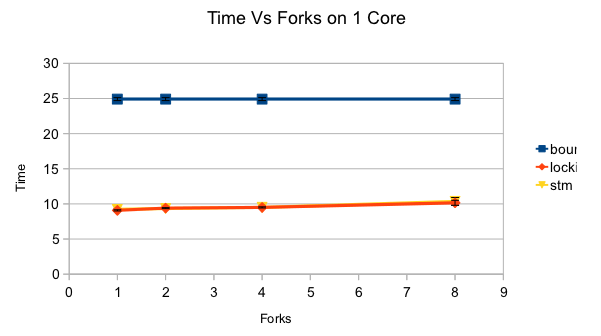
\includegraphics[width=\linewidth]{time-on-1-core.png}
\end{figure}
\begin{figure}[h]
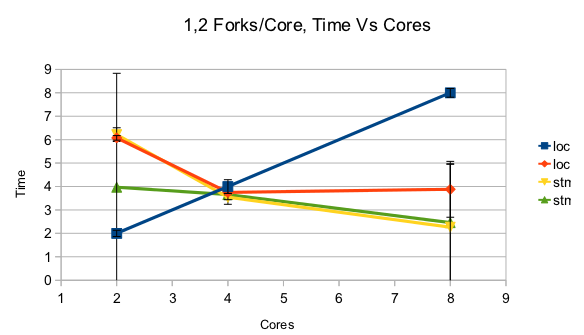
\includegraphics[width=\linewidth]{time-and-forks-on-cores.png}
\end{figure}
\begin{figure}[h]
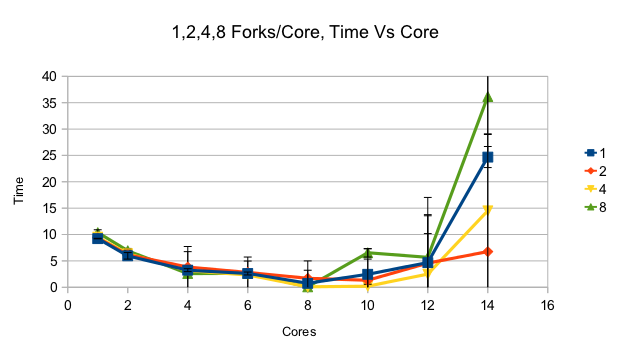
\includegraphics[width=\linewidth]{time-and-forks-on-cores-again.png}
\end{figure}
\begin{figure}[h]
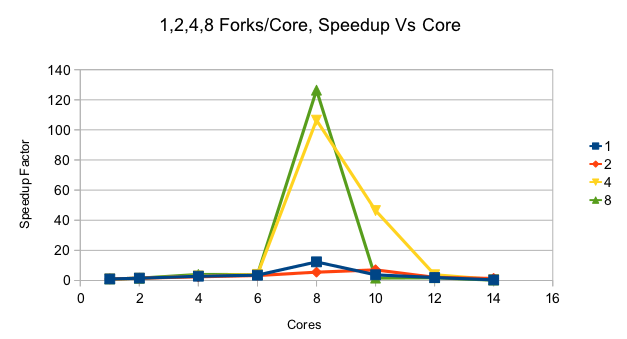
\includegraphics[width=\linewidth]{speedup-and-forks-on-cores.png}
\end{figure}
\begin{figure}[h]
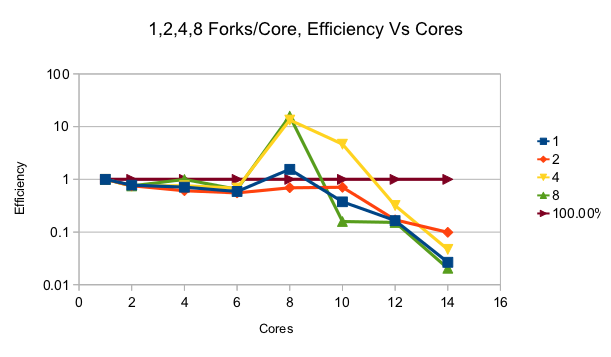
\includegraphics[width=\linewidth]{log-efficiency-and-forks-on-cores.png}
\end{figure}
\end{document}
